\section{Data Structures}
\label{sec:enclaves}

The central context of SGX is the \textit{enclave}, a protected environment
that contains the code and data pertaining to a security-sensitive computation.
This section provides an overview of the data structures used by an enclave.


\subsection{Enclaves and the RAM}

% PRM: SGX S 3.5

The enclaves' code and data is stored in \textit{Processor Reserved Memory}
(PRM), a contiguous range of RAM that cannot be directly accessed by other
software, including privileged software such as the SMM code, the hypervisor,
and the OS kernel. The CPU also prevents devices attached to the system bus
from performing DMA transfers to/from the PRM. This is possible because, on
modern systems, the northbridge is integrated into the CPU
(see Figure \ref{fig:pch}).

On systems with SGX-enabled CPUs, the BIOS is responsible for setting aside a
contiguous range of RAM for \textit{Processor Reserved Memory} (PRM). The
CPU prevents most programs (including the SMM handler, the hypervisor and the
operating system kernel) from accessing the PRM.


The PRM must be set up to use SGX features and, once configured, the PRM range
cannot be changed. Furthermore, the PRM's size must be an integer power of two,
and its start address must be aligned to the same power of two. The range
restrictions reduce the complexity of checking if a RAM address is in the PRM
to a bitwise AND and an equality comparison.

\begin{figure}[hbtp]
  \center{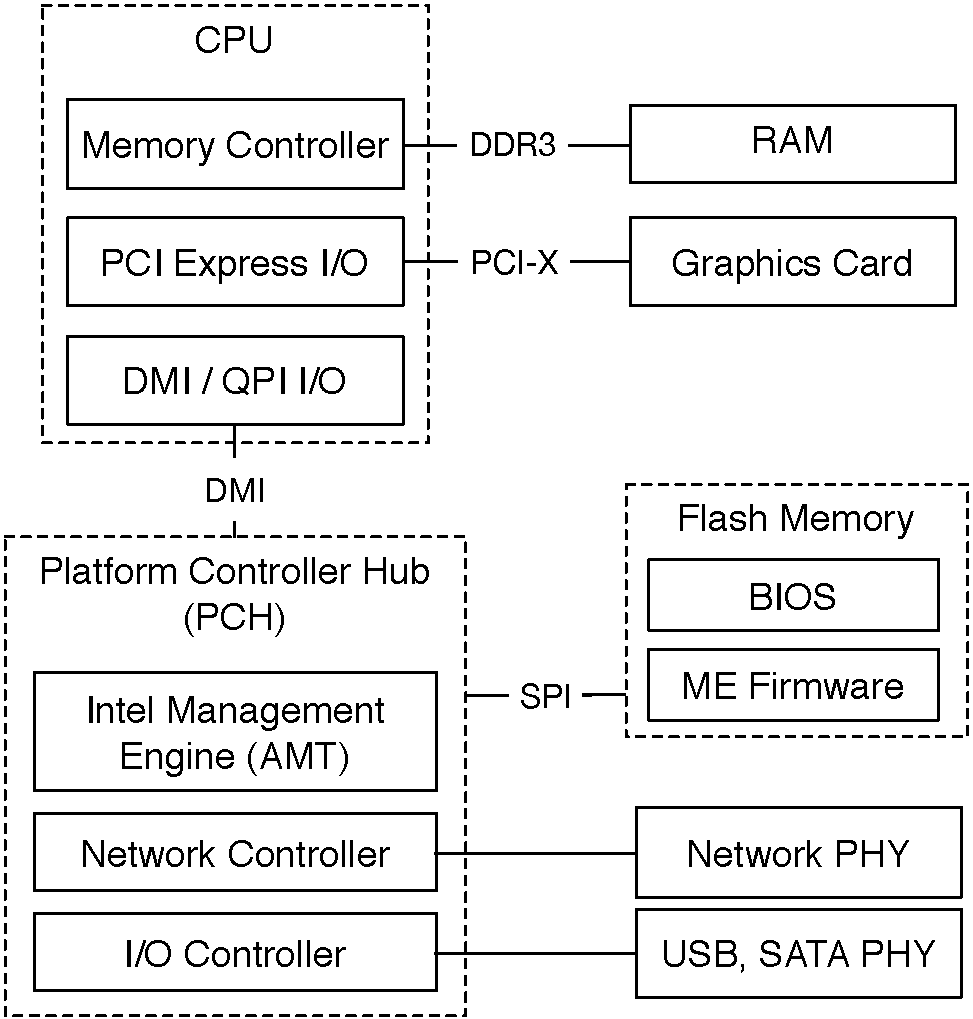
\includegraphics[width=65mm]{figures/pch.pdf}}
  \caption{
    The architecture of modern Intel systems.
    The Platform Controller Hub (PCH) contains a service processor, called the
    Intel Management Engine (ME). The processor has direct access to the
    network, can read and modify RAM via DMA transfers, and can override the
    CPU boot vector. The processor runs firmware stored in the same flash
    memory as the BIOS code.
  }
  \label{fig:pch}
\end{figure}

% EPC and EPCM: SGX S 1.5, S 1.5.1, S 2.6.13, S 3.5, S 3.5.1

The contents of enclaves and the associated data structures are stored in the
\textit{Enclave Page Cache} (EPC). The EPC is a subset of the PRM

, so the
protection measures described in the paragraphs above ensure that the enclaves'
memory cannot be read or tampered with by any malicious software running on the
host computer, or by malicious peripherals attached to the system bus. The
stringent restrictions placed on PRM documented above reduce the probability of
bugs in the security checks at the foundation for SGX's integrity and privacy
guarantees.

The EPC is split into 4kb pages, which are allocated to enclaves or supporting
data structures by the \textit{system software}, which can be either a
\textit{hypervisor} (the software running in VMX root mode at ring 0), or a
\textit{kernel} (the code inside an operating system running at ring 0).

The CPU maintains some metadata for each EPC page into the \textit{Enclave Page
Cache Map} (EPCM), which is used to ensure that an enclave does not attempt to
access another enclave's pages, and that system software manages EPC pages in a
way that is consistent with the SGX security model. The SGX documentation does
not state where the EPCM is stored, but we can hypothesize that it is either
an on-chip memory, like the L3 cache, or stored in a PRM region that is not
used by the EPC.

% SECINFO: SGX S 2.6.5, S 2.6.5.{1,2}

\subsection{Enclave Structures}

Each enclave has a \textit{SGX Enclave Control Structure} (SECS)


% SECS: SGX S 2.6.1, S 2.6.1.1,


% TCS: SGX S 2.6.2, S 2.6.2.{1,2,3,4}


% SSA: SGX S 2.6.3,
